Para garantizar el correcto funcionamiento de cada uno de los componentes se diseñan una serie de test para comprobar el comportamiento. Para esto se usará una librería llamada Jest \cite{jest} , para instalarla se debe ejecutar el siguiente comando.
\newline
\begin{figure}[H]
    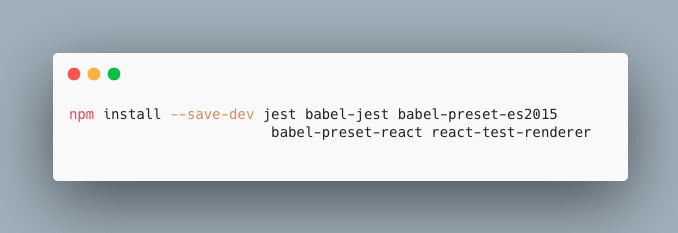
\includegraphics[width=1\textwidth]{./Imagenes/8.39t.png}
    \caption[Instalar dependencias]{Instalar dependencias}
    \end{figure}
\newline
Las dependencias instaladas con el comando anterior solo son usadas durante el desarrollo.

Dentro del directorio src debemos crear un subdirectorio llamado Test.
\newline
\begin{figure}[H]
    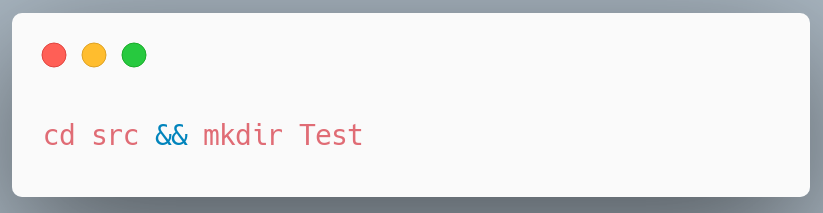
\includegraphics[width=1\textwidth]{./Imagenes/8.40t.png}
    \caption[Crear directorio]{Crear directorio}
    \end{figure}
\newline
Y dentro de este directorio crearemos un archivo por cada uno de los componentes llamado de la siguiente manera.
\begin{figure}[H]
   Nombre del Componente + . + test + . + js
    \centering
    \end{figure}
    
 Dentro de este se tendrán un código para asegurar el funcionamiento, por ejemplo para el componente Button se diseñó el siguiente test.
 \newline
\begin{figure}[H]
    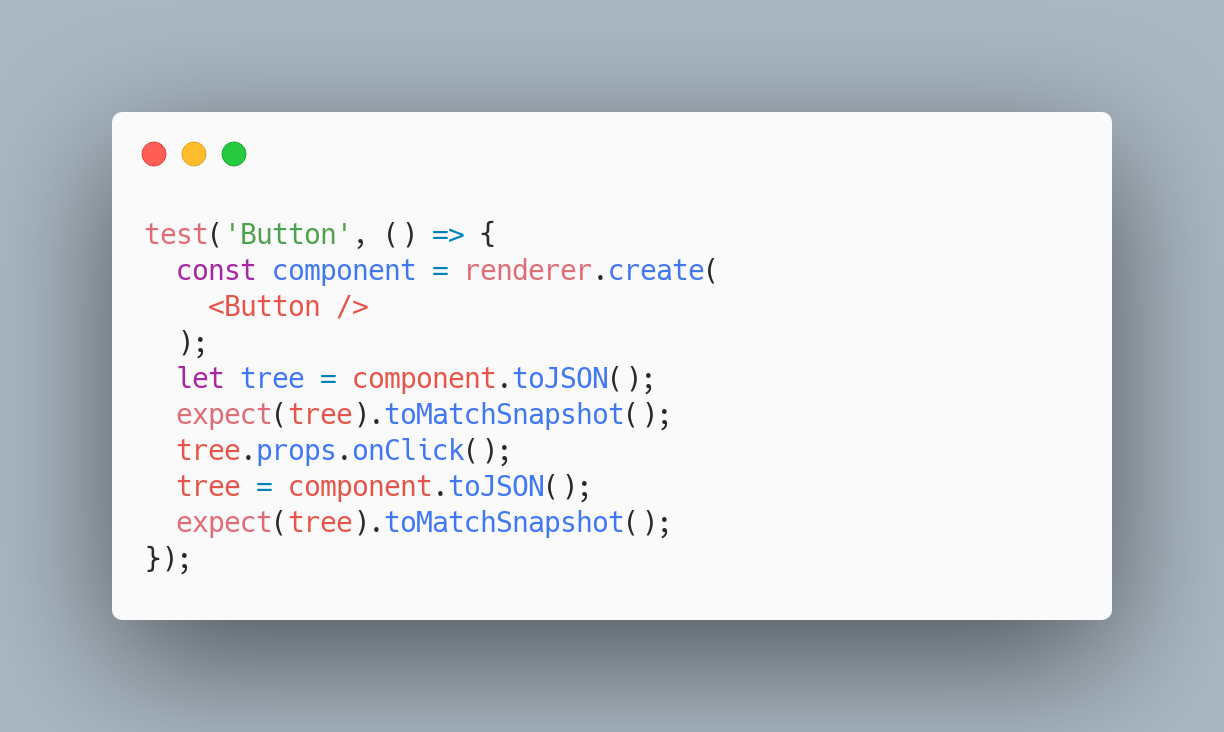
\includegraphics[width=1\textwidth]{./Imagenes/8.41t.png}
    \caption[Test del componente Button]{Test del componente Button}
    \end{figure}
\newline

El cual crea un componente, después crea una copia del resultado, y cada que se ejecute el test se debe comparar con la copia creada.
La segunda parte del test hacé click en el botón y verifica el funcionamiento.

Para poder ejecutar el todos los test, se debe agregar el siguiente comando en el archivo packeage.json.
 \newline
\begin{figure}[H]
    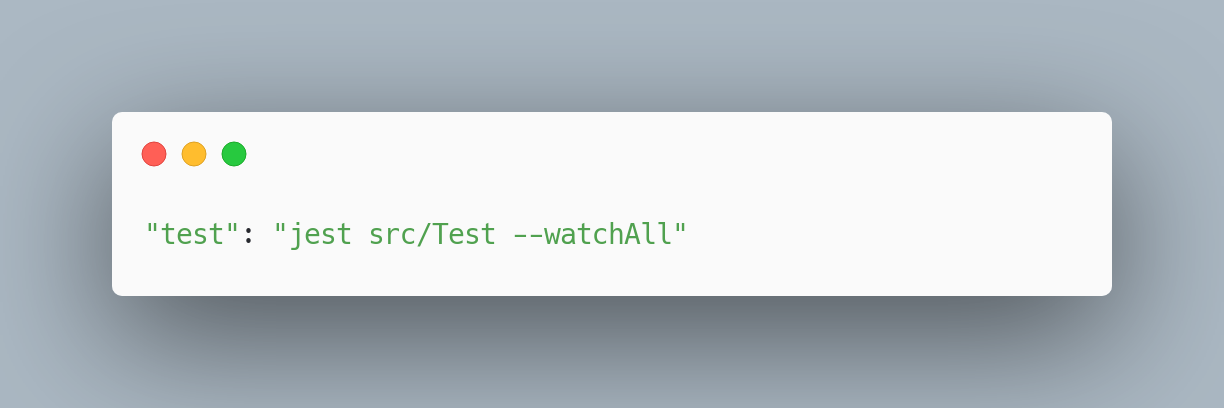
\includegraphics[width=1\textwidth]{./Imagenes/8.42t.png}
    \caption[Agregar comando]{Agregar comando}
    \end{figure}
\newline
\clearpage